\documentclass[a4paper]{article}
\usepackage[utf8]{inputenc}
\usepackage[russian,english]{babel}
\usepackage[T2A]{fontenc}
\usepackage[left=10mm, top=20mm, right=18mm, bottom=15mm, footskip=10mm]{geometry}
\usepackage{indentfirst}
\usepackage{amsmath,amssymb}
\usepackage[italicdiff]{physics}
\usepackage{graphicx}
\usepackage{multirow}
\usepackage{svg}
\graphicspath{{images/}}
\DeclareGraphicsExtensions{.pdf,.png,.jpg}
\usepackage{wrapfig}
\usepackage{caption}
\captionsetup[figure]{name=Рисунок}
\captionsetup[table]{name=Таблица}
\title{\underline{Амплитудная диффракционная решетка. Работа 4.4.1}}
\author{Каспаров Николай, Б01-304}

\begin{document}

\maketitle
\begin{center}
\Large{\textbf{ }}
\end{center}

\subparagraph{Цель работы:}

\begin{itemize}
    \item Знакомство с работой и настройкой гониометра Г5;
    \item Определение спектральных характеристик амплитудной решётки.
\end{itemize}

\subparagraph{В работе используются:}

\begin{itemize}
    \item Гониометр;
    \item Дифракционная решётка;
    \item Ртутная лампа.
\end{itemize}

\section{Теоретическое введение}

    \subsection{Основное соотношение}

    Наблюдение изображения спектра проводится с помощью зрительной трубы,
    настроенной на бесконечность.
    В этом случае амплитуда и интенсивность поля световой волны определяются углом $\phi$ между нормалью к решётке и направлением дифрагировавших лучей.
    Будем считать, что амплитуды всех интерферирующих волн одинаковы,
    т. е. фиксирована амплитуда падающей волны и постоянна площадь всех штрихов.
    Интенсивность дифрагированного света максимальна для углов $\phi_m$,
    при которых волны, приходящие в точку наблюдения от всех щелей, оказываются в фазе:

    \begin{equation}
        d \sin{\phi_m} = m \lambda
        \label{main_eq}
    \end{equation}
    Величина $m = 0, \pm 1, \pm 2, \pm 3, ...$ называется порядком спектра.

    \subsection{Угловая дисперсия}

    Выражение для угловой дисперсии дифракционной решётки следует из \eqref{main_eq}:

    \begin{equation}
        D = \frac{d\varphi}{d\lambda} = \frac{m}{d \cos \varphi}=\frac{m}{\sqrt{d^{2}-m^{2} \lambda^{2}}}.
    \end{equation}

    \subsection{Разрешающая способность}

    Рассмотрим изображения спектра для двух узких спектральных линий с длинами волн $\lambda$ и $\lambda+\delta\lambda$.
    Для минимального значения $\lambda+\delta\lambda$, которое может быть определено по результатам измерений, вводят важнейшую характеристику спектрального прибора — разрешающую способность:

    \begin{equation}
        R=\frac{\lambda}{\delta\lambda}.
        \label{razr}
    \end{equation}

\section{Экспериментальная установка}

\begin{figure}[!h]
    \centering
    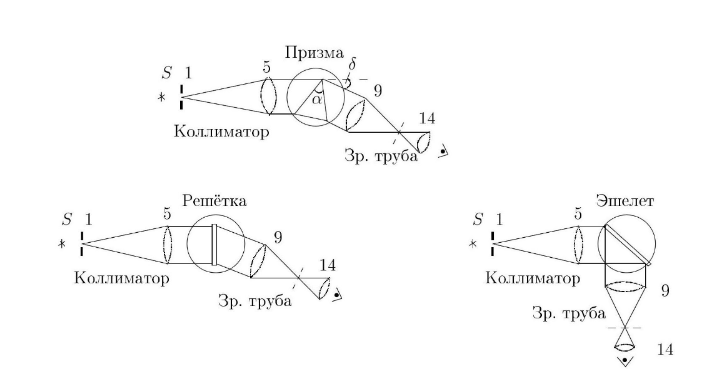
\includegraphics[width=0.8\textwidth]{Ustanovka.png}
    \caption{Экспериментальная установка}
    \label{fig:ustanovka}
\end{figure}

В данной работе будем измерять углы, при которых наблюдаются максимумы для разнычных длин волн. 
Схема экспериментальной установки представлена на рисунке \ref{fig:ustanovka}.

\newpage

\section{Экспериментальная часть}

\subsection{Определение параметров решетки}

\begin{table}[]
    \centering
    \begin{tabular}{|c|c|c|c|}
    \hline
    Цвет       & Порядок & d, нм & $\sin{\alpha}$ \\ \hline
    Синий      & 1       & 435.8 & 0.220          \\ \hline
    Голубой    & 1       & 491.6 & 0.248          \\ \hline
    Фиолетовый & 1       & 404.7 & 0.203          \\ \hline
    Зеленый    & 1       & 546.1 & 0.275          \\ \hline
    Желтый 1   & 1       & 577.0 & 0.292          \\ \hline
    Желтый 2   & 1       & 579.1 & 0.292          \\ \hline
    Красный    & 1       & 623.4 & 0.314          \\ \hline
    \end{tabular}
    \caption{Зависимость угла максимума от длины волны}
    \label{tab:my-table}
\end{table}

\begin{figure}[!h]
    \centering
    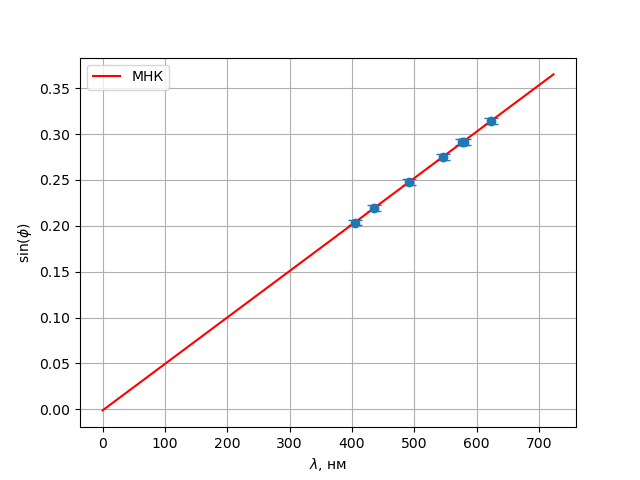
\includegraphics[width=0.6\textwidth]{fit_result.png}
    \caption{Зависимость угла максимума от длины волны}
    \label{fig:fit_result}
\end{figure}

\newpage

Вычислив угол наклона, мы сможем определить шаг решетки $d$, используя формулу \eqref{main_eq}:

\begin{equation}
    d = (1.96 \pm 0.04) \ \text{мкм},
\end{equation}
что совпадает на значение, указанное на приборе: $d_{th} = 2$ мкм.

\subsection{Определение угловой дисперсии}

\begin{table}[!h]
    \centering
    \begin{tabular}{|c|c|c|}
    \hline
    Порядок & $\phi$ & $\Delta \phi$ \\ \hline
    1       & 16°56$'$ & $ 2'20''$   \\ \hline
    2       & 35°59$'$ & $10'00''$   \\ \hline
    3       & 60°39$'$ & $20'36''$   \\ \hline
    \end{tabular}
    \caption{Зависимость разности угла желтого цвета от её порядка}
    \label{tab:angles}
\end{table}

\begin{figure}[!h]
    \centering
    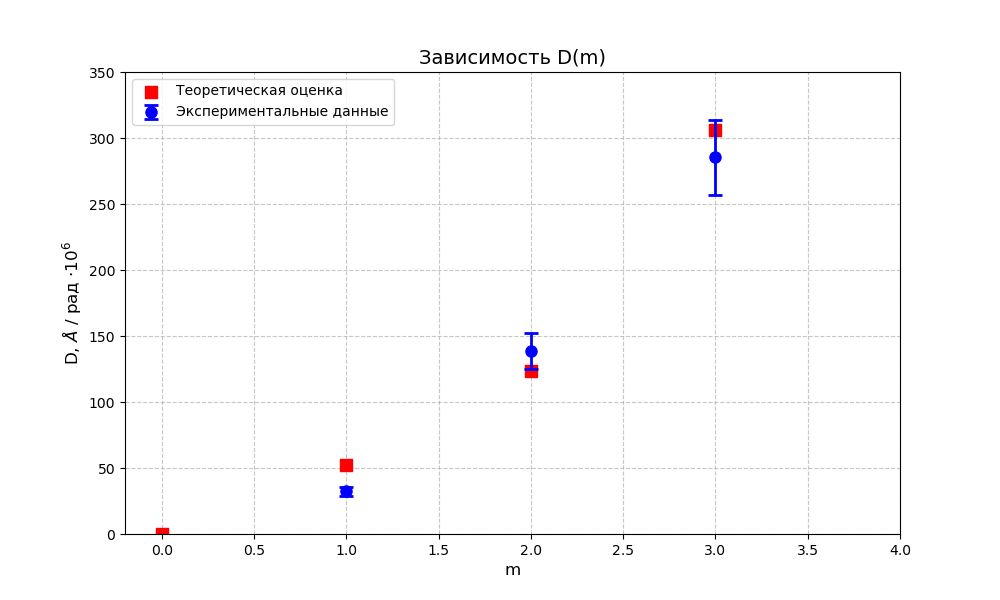
\includegraphics[width=0.8\textwidth]{approx2.png}
    \caption{Угловая дисперсия для разных порядков}
\end{figure}

Из-за малости разности углов, получилась достаточно высокая погрешность.

\subsection{Определение разрешающей способности}

Определим также разрешающую способность по формуле \ref{razr},
используя первый порядок жёлтой линии:

\begin{equation}
    R = 510 \pm 10
\end{equation}

Число рабочих штрихов $N = m \cdot R = 510 \pm 10 $,
а размер освещенной части $l = Nd = (1.0 \pm 0.1) \ \text{мм}$

\section{Вывод}

В ходе работы была исследована амплитудная дифракционная решётка, определены её спектральные характеристики, угловая дисперсия и разрешающая способность. Полученные значения шагa решётки и разрешающей способности согласуются с теоретическими данными в пределах погрешности. При более аккуратных измерениях можно добиться ещё большей точности результатов.

\end{document}
